\section{Testes}

\par Esta secção divide-se em duas subsecções, a primeira diz respeita a refactoring e identificação de Code Smells\footnote{} e a segunda prende-se com testes feitos á aplicação para testar a sua robustez.

\subsection{Refactoring e Code Smells}

\par Para realizar o processo de code coverage foi usado o módulo Devel::Cover, este módulo permite correr um programa com os respetivos argumentos e monitorizar que partes do código foram usadas ou não foram usadas, criando posteriormente um relatório em html que permite visualizar de uma forma mais clara o desempenho do programa.
\par Para utilizar o Devel::Cover com o nosso programa e posteriormente criar o relatório pretendido basta correr os seguintes comandos pela ordem apresentada:
\begin{itemize}
	\item perl -MDevel::Cover signpdf\_cli.pl -u '+351 XXXXXXXXX' -p XXXX -infile teste.pdf -d
	\item cover
\end{itemize}

Após o programa terminar de executar podemos verificar que foi criada uma base de dados \textit{cover\_db} e que a informação da mesma foi compilada num relatório html.
O resultado de correr o teste\footnote{Note-se que a utilização do -d não é obrigatória mas foi usado para cobrir a maior parte do código possível.} é apresentado em seguida:

\begin{figure}[H]

  \centering
  \captionsetup{justification=centering}

  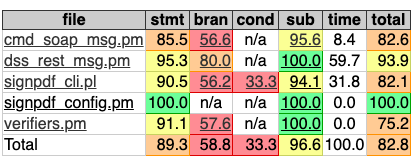
\includegraphics[scale = 0.25]{coverage1.png}
  
  \caption {Resultado de correr o programa utilizando o módulo Devel::Cover}

\end{figure}


\par Analisando a imagem anterior, verificamos que existem várias colunas na tabela, cada coluna tem o seguinte significado da esquerda para a direita: número de linhas do código utilizadas,nº de branches(if/else) utilizados\footnote{O número ótimo de branches utilizados é de 50\% uma vez que quando o código chega a um if then else segue apenas 1 dos caminhos possíveis, no entanto existem partes do código que possuem apenas um if ou que possuem subrotinas que não foram chamadas que possuem ifs, estes ifs contam para esta percentagem como não tendo sido avaliados, fazendo o valor final descer.}, percentagem das condições (as condições são compostas por elementos conjugados com as palavras \textit{and} e \textit{or}) avaliadas de forma positiva ou negativa, percentagem de subrotinas usadas, tempo em segundos que as subrotinas de cada ficheiro demoraram a executar.
\par Ao analisarmos os ficheiros para verificarmos que "statements" não estão a ser utilizados no código podemos verificar que estes se encontram todos dentro de condições if then else, sendo que como o programa correu bem, os statements não utilizados se encontram dentro dos else. Analisando a utilidade dos "statements" dentro do else constatamos que na sua maioria se tratam de comandos \textit{die} com informação sobre o porquê do programa ter sido interrompido naquele estágio.


\par Passando agora á análise dos branches do programa, devemos analisar para cada ficheiro se os branches são necessários, se as condições para que se siga por cada um dos caminhos das biforcações se manifestam. Tomemos por exemplo o relatório referente ao ficheiro \textit{cmd\_soap\_msg.pm}.

\begin{figure}[H]

  \centering
  \captionsetup{justification=centering}

  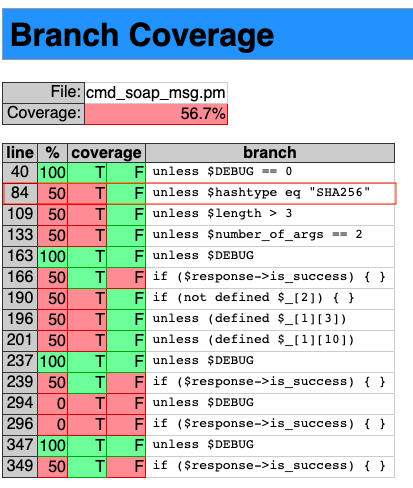
\includegraphics[scale = 0.25]{SOAPcoverage2.png}
  
  \caption {Relatório de branches do ficheiro cmd\_soap\_msg.pm}

\end{figure}

\par Após verificarmos a validade de cada branch, podemos observar que há um branch que não faz sentido porque verifica se um valor foi recebido, sendo que esse valor é passado de forma estática a essa função. Esse branch foi assinalado a vermelho para facilitar o seu reconhecimento. Podemos então apagar esse branch uma vez que não tem utilidade no código. O mesmo processo foi aplicado a cada ficheiro.

\par Podemos ainda ver que existe uma condição no código. O módulo Devel:Cover cria também um relatório para as condições do programa como se pode ver na imagem abaixo.

\begin{figure}[H]

  \centering
  \captionsetup{justification=centering}

  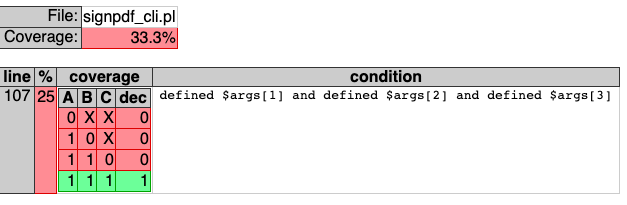
\includegraphics[scale = 0.25]{condition.png}
  
  \caption {Relatório de condições do ficheiro signpdf\_cli.pl}

\end{figure}

Podemos verificar que são mostradas as vária verificações que podem ser levadas a cabo e os respetivos resultados. Estes resultados são todos possíveis porque até aquele ponto não existe verificação se os 3 elementos que o cliente tem de fornecer ao programa são realmente fornecidos.
\par De facto, após a remoção de um if que se encontrava a mais no código este não apresenta mais nenhum tipo de código inutil, confuso, muito extenso ou duplicado.

\par Agora que removi os code Smells do código vou usar uma biblioteca chamada Perl::Critic que avalia o código fonte de acordo com as diretrizes do livro Perl Best Practices, além de outras métricas, como complexidade ciclomática. Este módulo permite escolher 5 tipos de severidade de problemas no código, podendo as falhas mais severas representar problemas que permitam que um utilizador mal intencionado se aproveite do nosso programa e as falhas mais ligeiras apenas questões de legibilidade do código. Por esta razão começamos por definir uma severidade de grau 4, desta forma apenas foram apresentados os erros mais graves, de severidade 5, a vermelho e os segundos mais graves, de severidade 4\footnote{Por questões de simplicidade de apresentação apenas é apresentado o resultado da aplicação do módulo ao ficheiro signpdf\_cli.pl, no entanto ressalva-se que o mesmo processo foi aplicado aos restantes ficheiros do programa.}, a laranja.

\begin{figure}[H]

  \centering
  \captionsetup{justification=centering}

  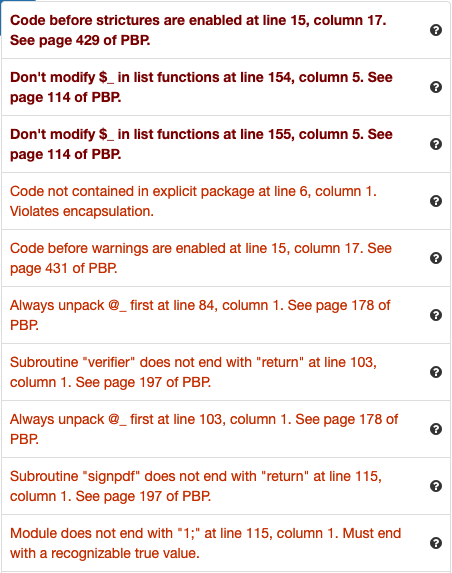
\includegraphics[scale = 0.3]{critic1.png}
  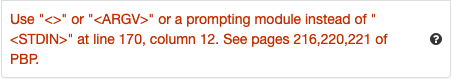
\includegraphics[scale = 0.3]{critic2.png}
  
  \caption {Relatório Perl::Critic de gravidades 4 e 5 do ficheiro signpdf\_cli.pl}

\end{figure}

\par As 3 primeiras notificações apresentadas correspondem a problemas criticos no código perl que foram resolvidos adicionando, após a adição do último módulo necessario, \textit{use strict;} para a primeira notificação e para as restantes duas bastou substituir o map que estava a modificar uma lista de certificados através do regex pela subrotina \textit{apply()} do módulo \textit{List::MoreUtils}. 
\par As restantes notificações possuem severidade 4. A primeira notificação refere-se á não identificação do código atual como um package, notificação essa que foi prontamente resolvida indicando na primeira linha do código \textit{package signpdf\_cli;}. A segunda notificação desapareceu com a adição do "use strict;".
\par Duas das notificações referiam que se trata de uma boa prática copiar o array recebido por uma subrotina, uma vez que caso este seja alterado dentro da subrotina, essa alteração notar-se-á na subrotina que a invocou. Adicionalmente 3 outras notificações foram resolvidas adicionando \textit{return 1;} ao final de todas as subrotinas que ainda não o possuiam e \textit{1;} o final do ficheiro, visto que os ficheiros e perl devem acabar com um valor de verdade.
\par Por fim o uso de \textit{<STDIN>} foi substituido pelo uso do \textit{prompt} pertencente ao módulo \textit{IO::Prompt}.

Como todas as notificações para uma análise de gravidade 4 pareciam importantes, decidi diminuir o filtro de gravidade da análise do ficheiro para 3 e o resultado obtido pode-se ver na imagem abaixo.

\begin{figure}[H]

  \centering
  \captionsetup{justification=centering}

  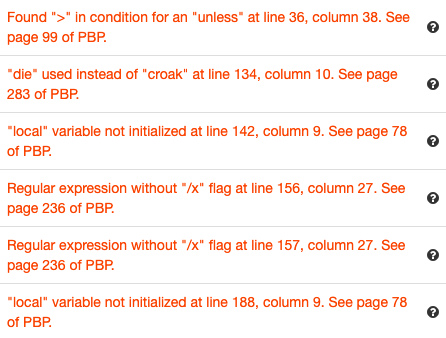
\includegraphics[scale = 0.3]{critic3.png}
  
  \caption {Segundo relatório Perl::Critic de gravidade 3 do ficheiro signpdf\_cli.pl}

\end{figure}

\par Estes erros são meramente para melhorar a simplicidade aciclomática do código, ou a legibilidade do mesmo, por esse motivo apliquei as mudanças requeridas ao ficheiro.
\par A primeira notificação referia que ao usar o simbolo de > dentro de um unless implicava uma dupla negativa, assim foi modificado o código, trocando o unless por um if.
\par A segunda notificação apenas pretende assinalar que quando nos deparamos com um erro de input por parte do utilizador, não devemos usar o comando \textit{die} que serve para reportar erros da aplicação mas o comando \textit{croak} que serve explicitamente para assinalar que o erro foi de um terçeiro não da aplicação.
\par A terceira e quinta notificações dizem respeito á legibilidade do código, apesar de quando se declara apenas uma variável sem lhe atribuir qualquer valor esta ser indefinida, devemos indicar explicitamente isto atribuindo-lhe o valor \textit{undef}.
\par Por fim é referido que a expressão \textit{s/\textbackslash s*-----\textbackslash s*BEGIN CERTIFICATE\textbackslash s*-----\textbackslash s*//} é demasiado grande e deve ser dividida para que se possão acrescentar comentários a cada parte para que se perceba o que se está a passar, no entanto, este erro deve-se á adição dos \textit{\textbackslash s*} algo que a meu ver não influencia a legibilidade, adicionalmente separar este regex tornalo-ia mais confuso do que está atualmente uma vez que este pretende representar uma string be mcompacta e curta sendo os \textit{\textbackslash s*} adicionados apenas uma medida de precaução.
\hfill\newline
\par Adicionalmente, foi criado um script perl chamado \textit{tester.pl} que utiliza o módulo \textit{Test::Vars} para garantir que não existem variáveis por usar no programa. O resultado de correr este script sobre os ficheiros do programa é o seguinte:

\begin{figure}[H]

  \centering
  \captionsetup{justification=centering}

  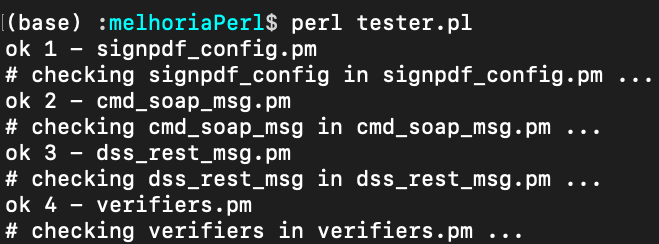
\includegraphics[scale = 0.25]{testvars.png}
  
  \caption {Segundo relatório Perl::Critic do ficheiro signpdf\_cli.pl}

\end{figure}


\subsection{Testes}

\par Para realizarmos testes sobre a aplicação, temos de verificar de que forma a podemos comprometer. A forma que temos de tentar realizar um ataque é através da inserção de inputs maliciosos, que podem ser introduzidos quando se passam argumentos no inicio programa ou no seu decorrer ou então quando o programa recebe uma resposta do servidor.























